系统采用py语言编程,软件使用主控模块树莓派定制版本,将程序模块化,便于功能的进一步扩展,模块化还有利于错误的检查和后期的优化。完整的停车管理系统的道闸设计包含主程序的设计、拍照模块的程序设计、驱动模块的程序设计。

\subsubsection{主程序模块的设计}

主控模块通电后立即进入系统并且连接上WiFi无线网络,在搭建好运行环境以及经过代码调试之后,启动进车程序。在进车程序中,车缓缓停下准备入库。若此时第一个红外检测到车身经过,则摄像头开启抓捕拍照,而且仅仅拍一张照片,将其存放到树莓派本地。紧接着照片被送往云端识别,会立即返回车的车牌号码。可能会出现未识别的情况,只要车不退回,系统会一直拍照直至能够产生车牌号码,除非用户自己离开系统放弃拍照。若产生正确的照片会被发往停车管理系统云端,返回剩余车位不为0时则杆立即抬起,车开始开进车库,第二个红外模块检测到车身时直至检测不到杆落下。整个进库的流程图如图\ref{fig:车入库主程序流程图}所示。

\begin{figure}[htbp]
	\centering
	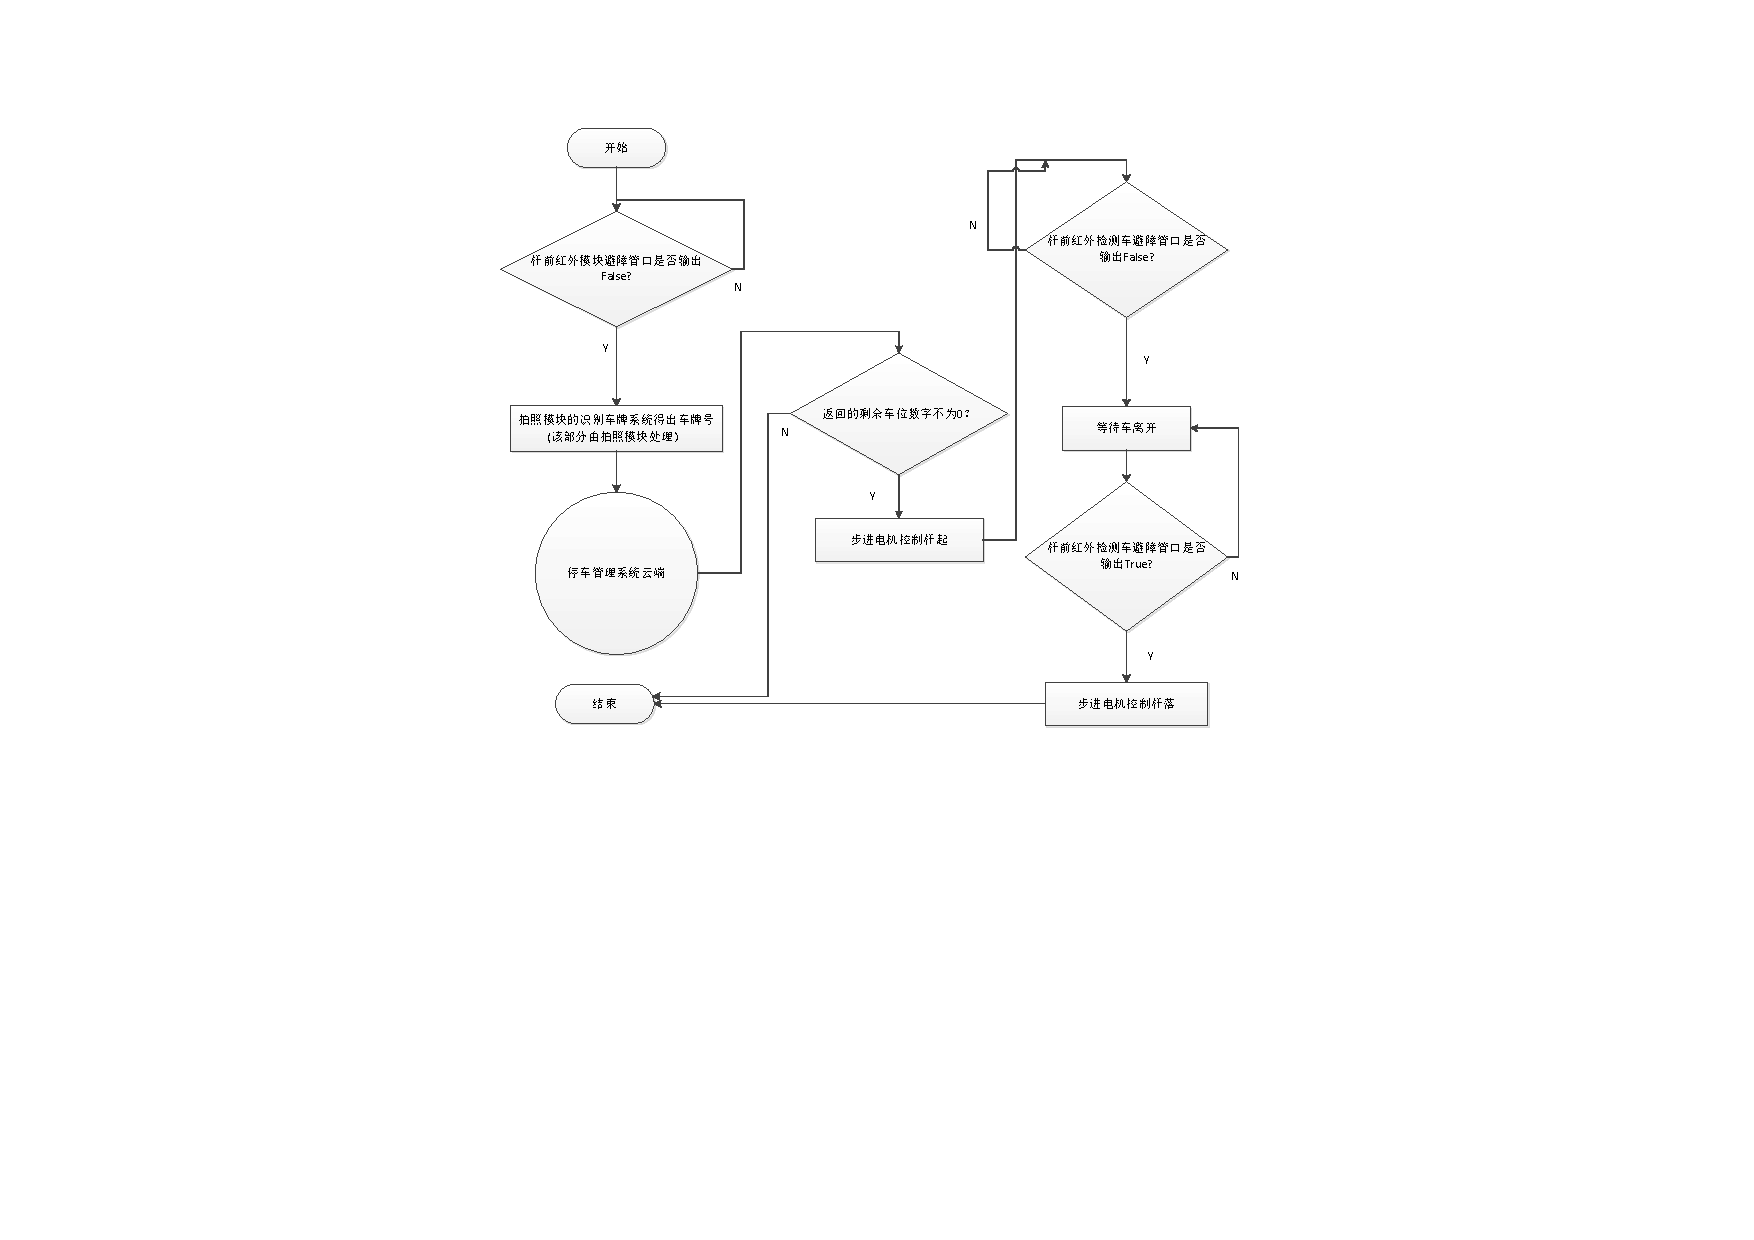
\includegraphics[width=\textwidth]{figure/software-1.pdf}
	\caption{车入库主程序流程图}\label{fig:车入库主程序流程图}
\end{figure}

出库程序运行时,当红外模块检测到车身时,则摄像头开启抓捕拍照。类似于车进库的操作,照片被送往云端识别,云端会返回车的号码。若是没有识别会会一直识别,若是长久不能识别,车主此时必须打电话给管理员。若是车牌识别成功,会立即发往停车管理系统云端,云端返回一个SVG字符串格式的二维码。
在本地将此格式转换为jpg图片格式即为付款二维码。车主需要付款扫二维码并付款成功后杆才可抬起,离开的时候第二个红外模块第一次检测到车身不落杆,直到避障管脚输入True时,杆才开始落下,此时车已经安全离开。车出库主程序流程图如图\ref{fig:车出库主程序流程图}所示。
 
\begin{figure}[htbp]
	\centering
	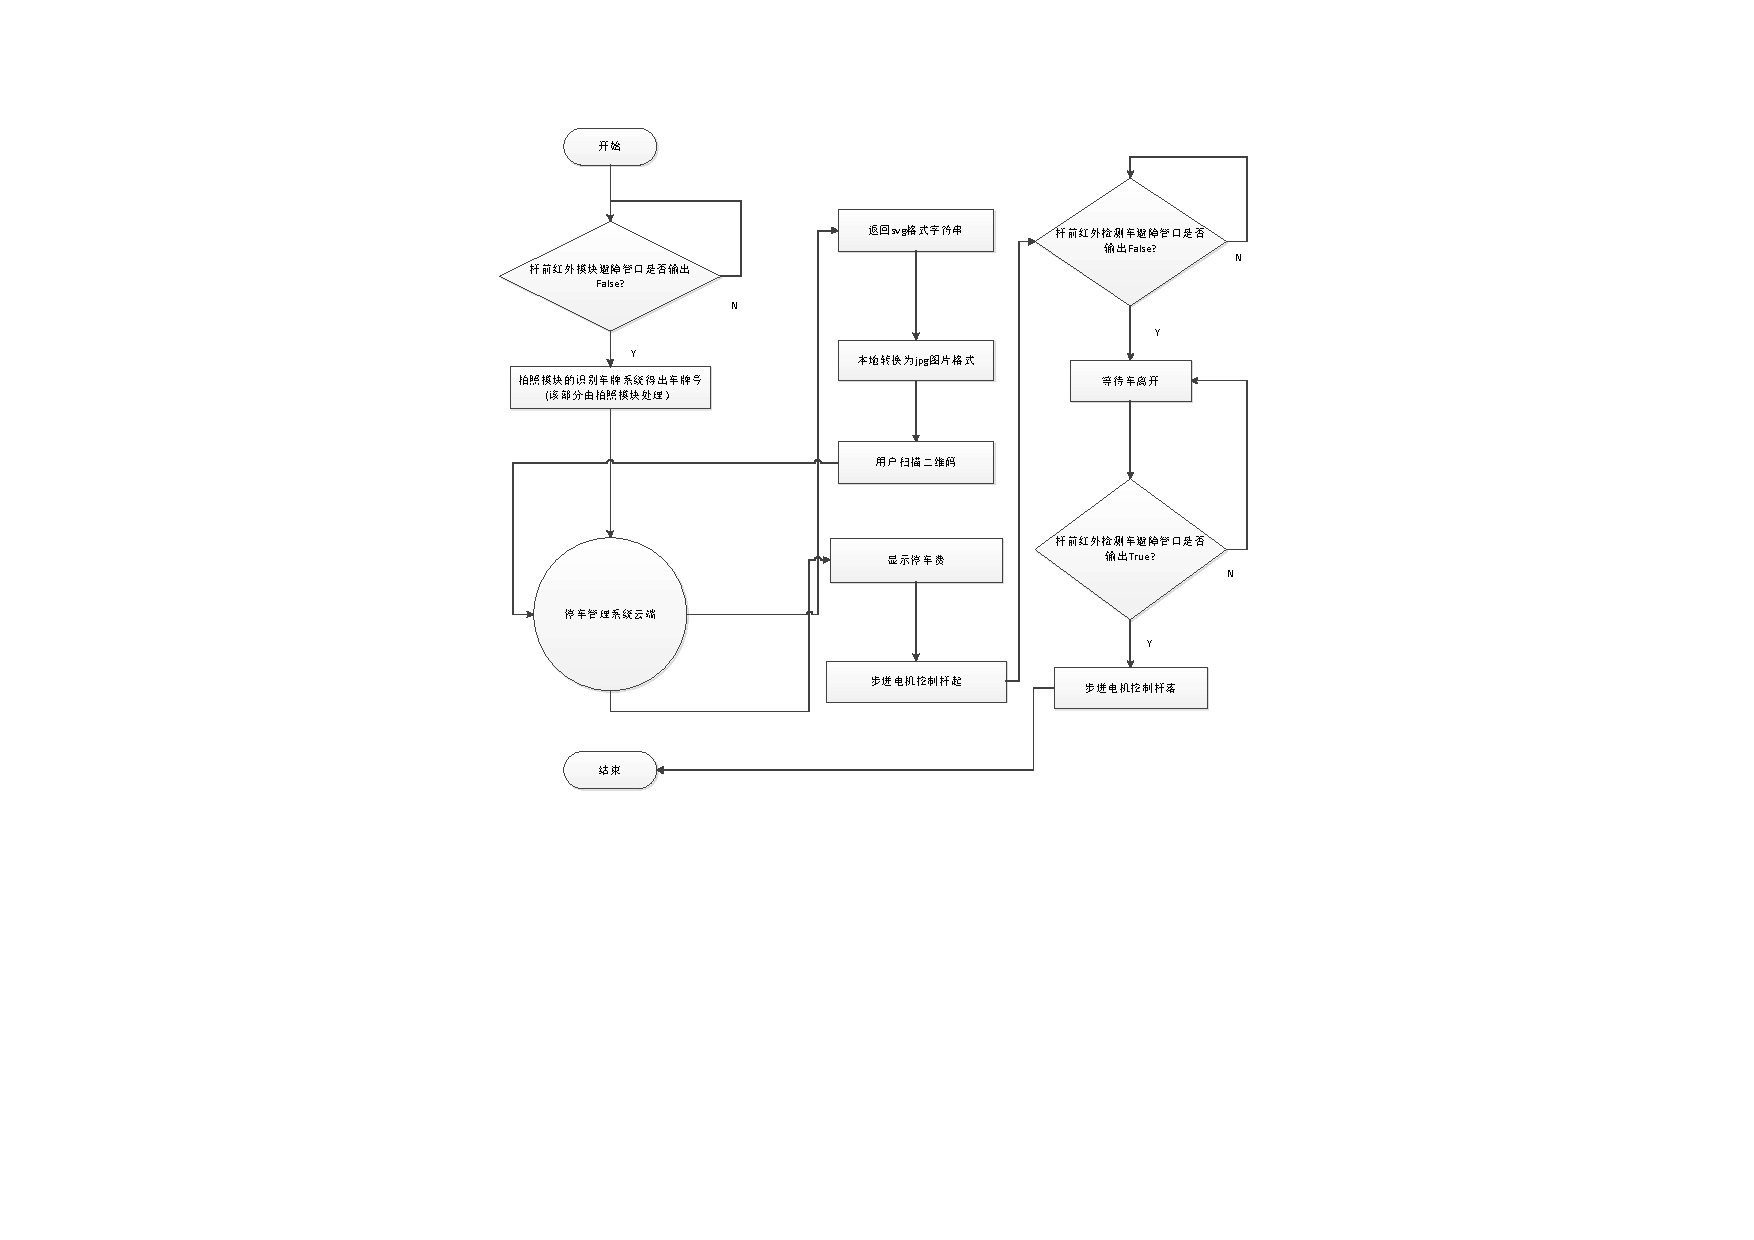
\includegraphics[width=\textwidth]{figure/software-2.pdf}
	\caption{车出库主程序流程图}\label{fig:车出库主程序流程图}
\end{figure}

\subsubsection{拍照模块的设计}
车进库初次进入系统将拍照模块功能设置为enabled,以便程序调用。在本次的设计中,程序本想利用OpenCV进行照片的处理,但因为网络的问题无法下载OpenCV程序包,故利用云端识别的方法从云端返回识别的图片。调用进行拍照处理。当拍照模块的拍照服务启动时,将采集的图片保存为jpg格式,然后等待下次调用拍照模块程序设计流程图如图\ref{fig:入库拍照模块程序设计流程图}所示。
 
\begin{figure}[htbp]
	\centering
	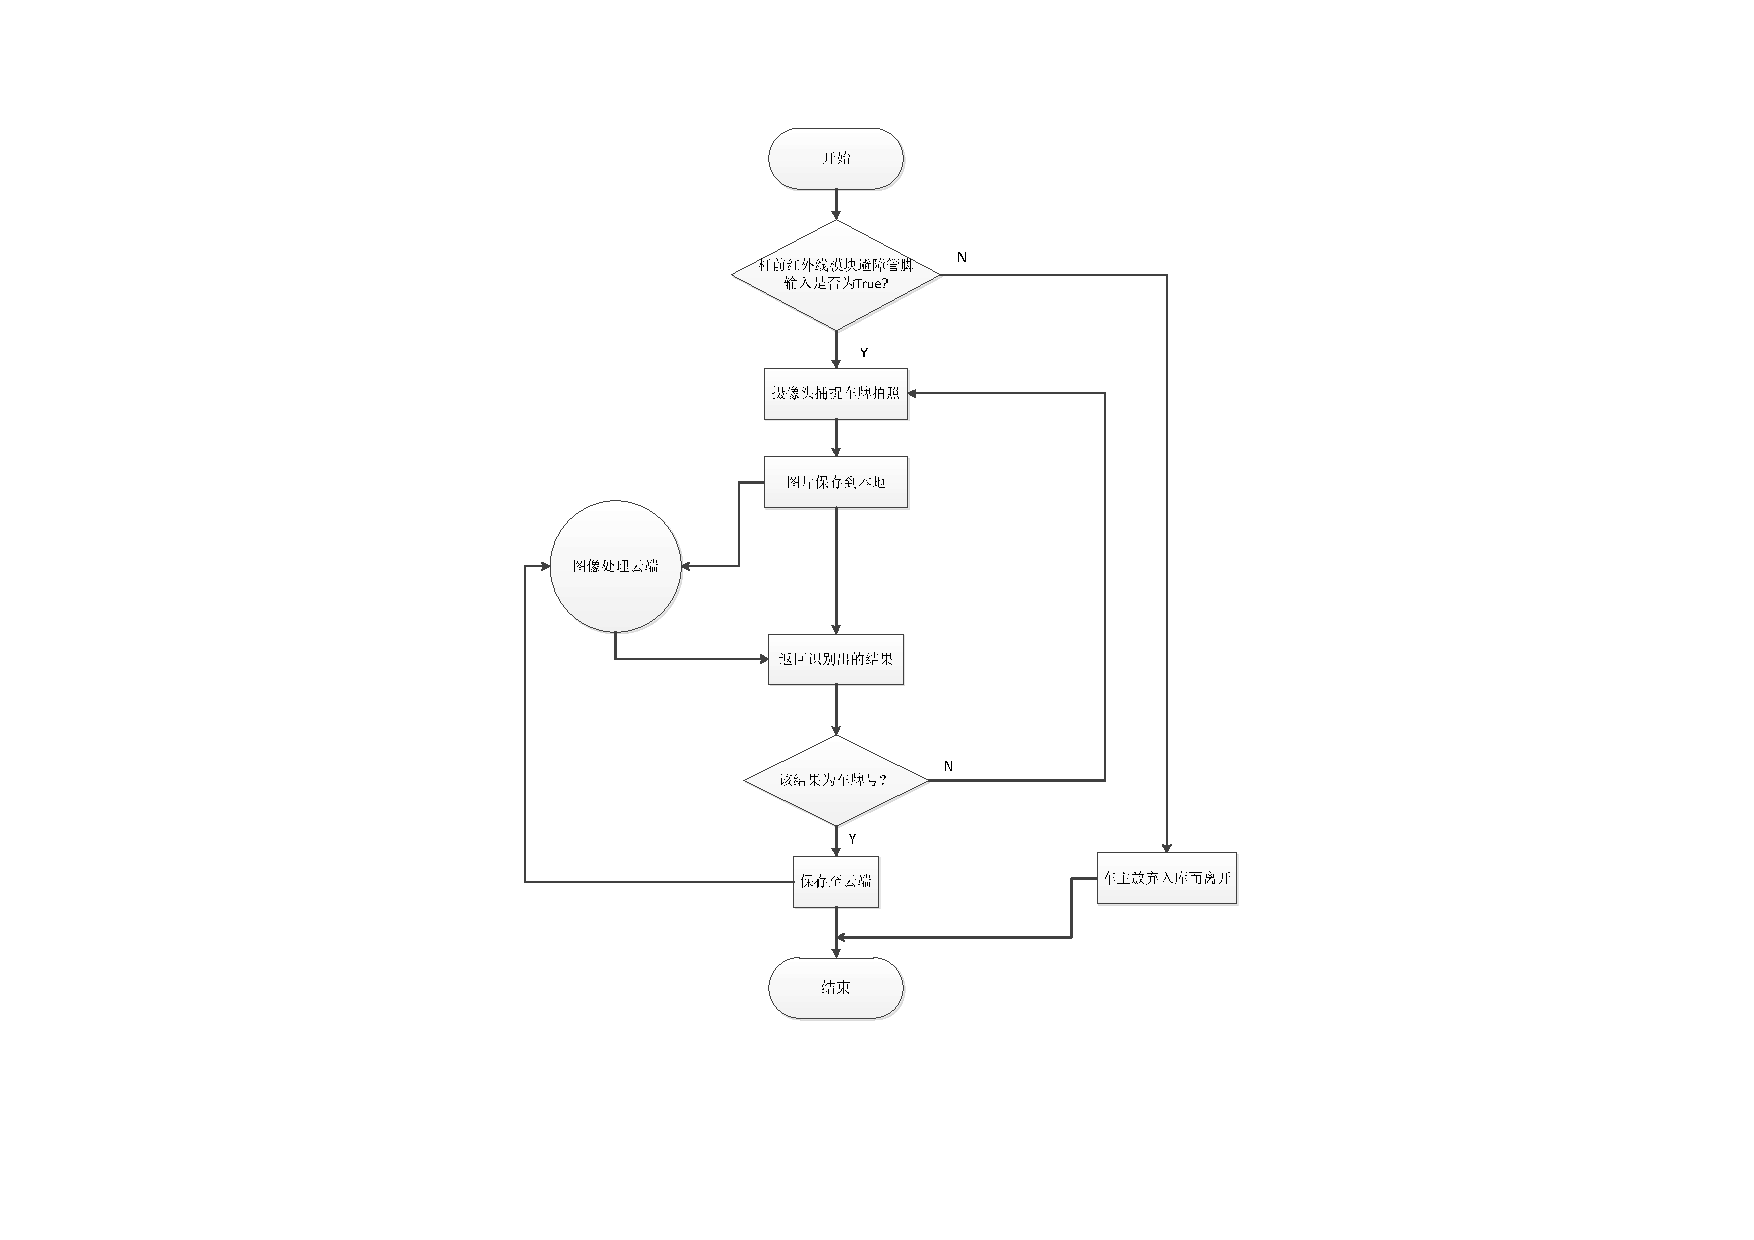
\includegraphics[width=\textwidth]{figure/software-3.pdf}
	\caption{入库拍照模块程序设计流程图}\label{fig:入库拍照模块程序设计流程图}
\end{figure}

车出库与进库拍照模块程序基本一致,有一点不一样,车入库时若是照片一直无法识别,车主可以选择离开,大不了换其他停车场。但是若是出库时照片识别不,车主只能打电话给管理员。出库拍照模块程序设计流程图如图\ref{fig:出库拍照模块程序设计流程图}所示。

\begin{figure}[htbp]
	\centering
	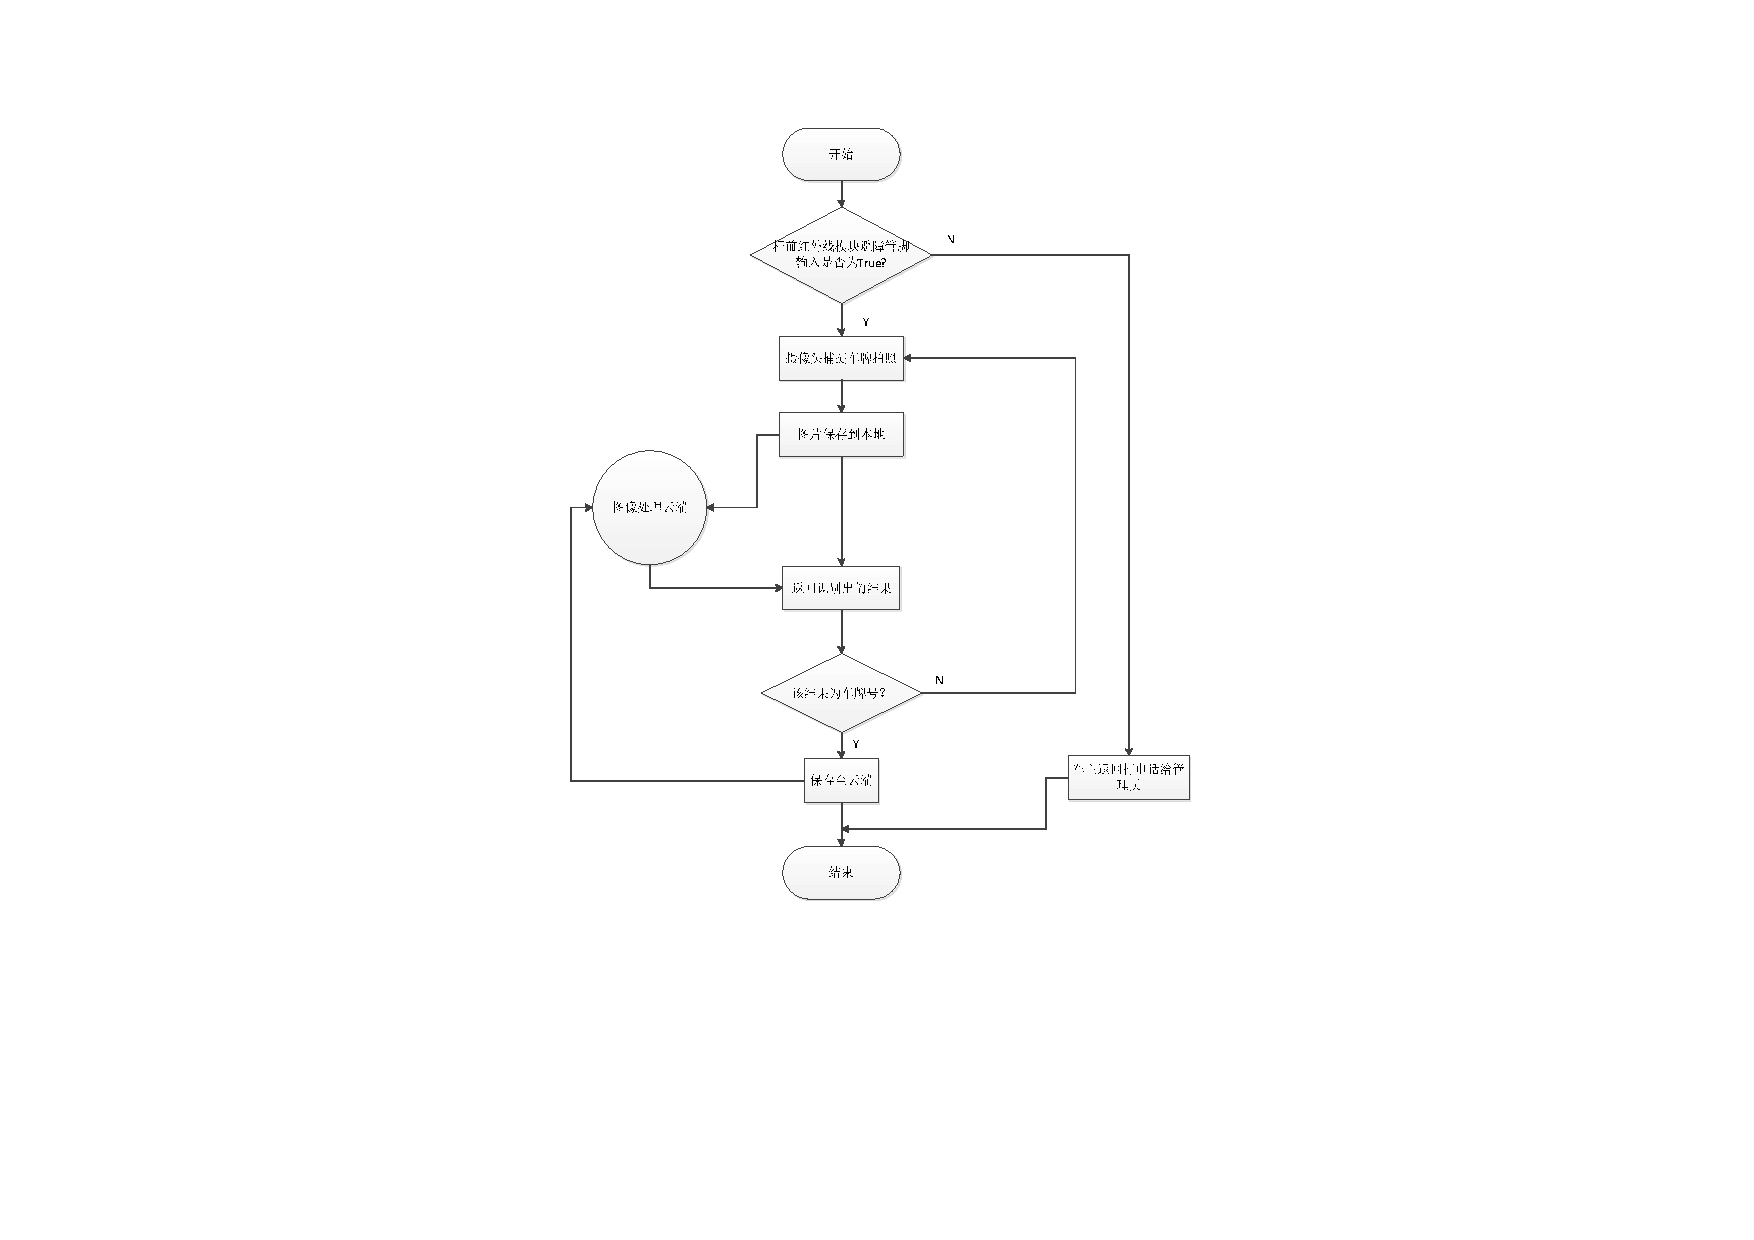
\includegraphics[width=\textwidth]{figure/software-4.pdf}
	\caption{出库拍照模块程序设计流程图}\label{fig:出库拍照模块程序设计流程图}
\end{figure}

\subsubsection{驱动模块的设计}
为了驱动步进电机首先设置主控模块相应的引脚为OutPut模式。主控模块中通过驱动模块带动步进电机旋转,进库时电机起杆(也即电机逆时针旋转90度)。电机在车入库时起杆的最终触发程序是停车管理系统云端显示还有剩余车位,落杆的最终条件是第二个红外模块检测不到车身。入库驱动模块设计流程如图\ref{fig:入库驱动模块设计流程图}所示。

\begin{figure}[htbp]
	\centering
	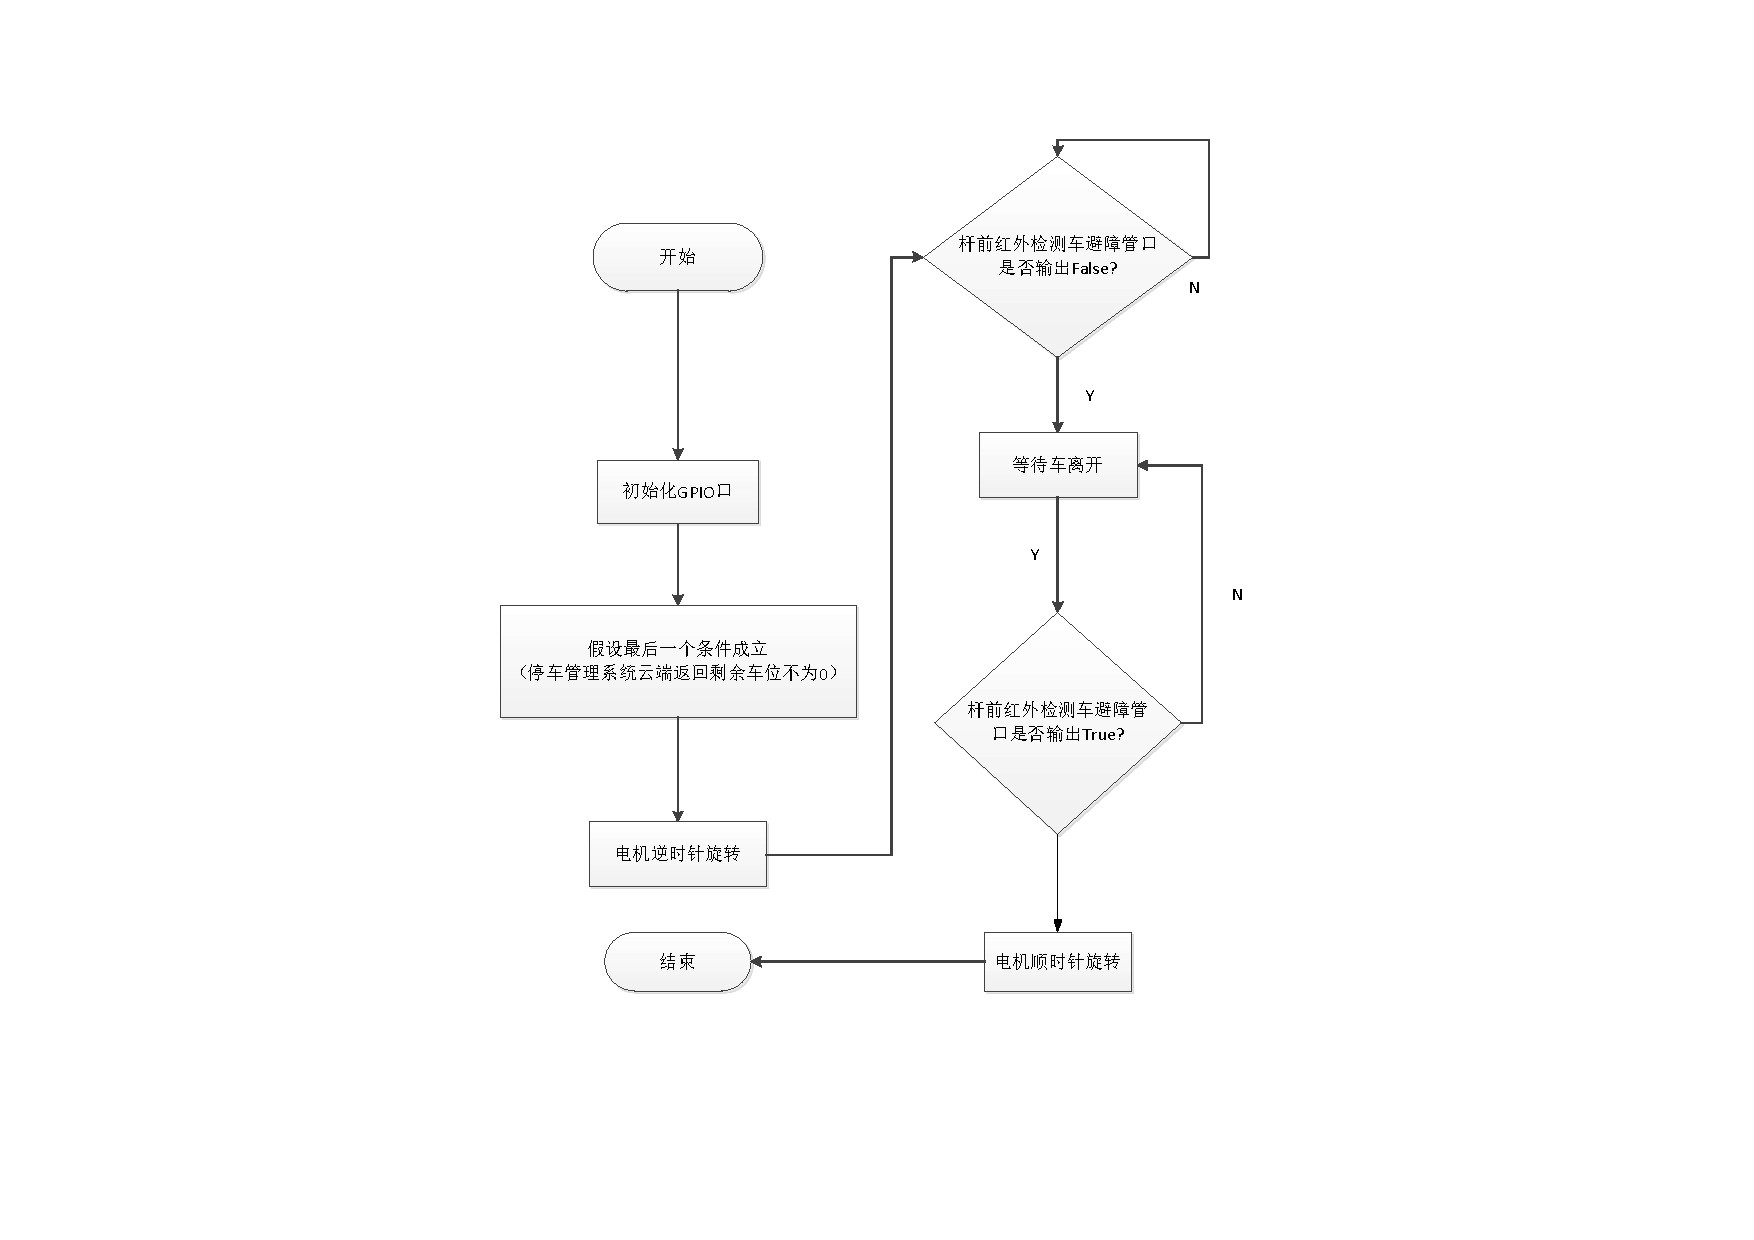
\includegraphics[width=\textwidth]{figure/software-5.pdf}
	\caption{入库驱动模块设计流程图}\label{fig:入库驱动模块设计流程图}
\end{figure}

电机在车出库时起杆的最终条件是车主付款成功,而落杆的最终条件与车入库完全一样。出库驱动模块设计流程图如图\ref{fig:出库驱动模块设计流程图}所示。

\begin{figure}[htbp]
	\centering
	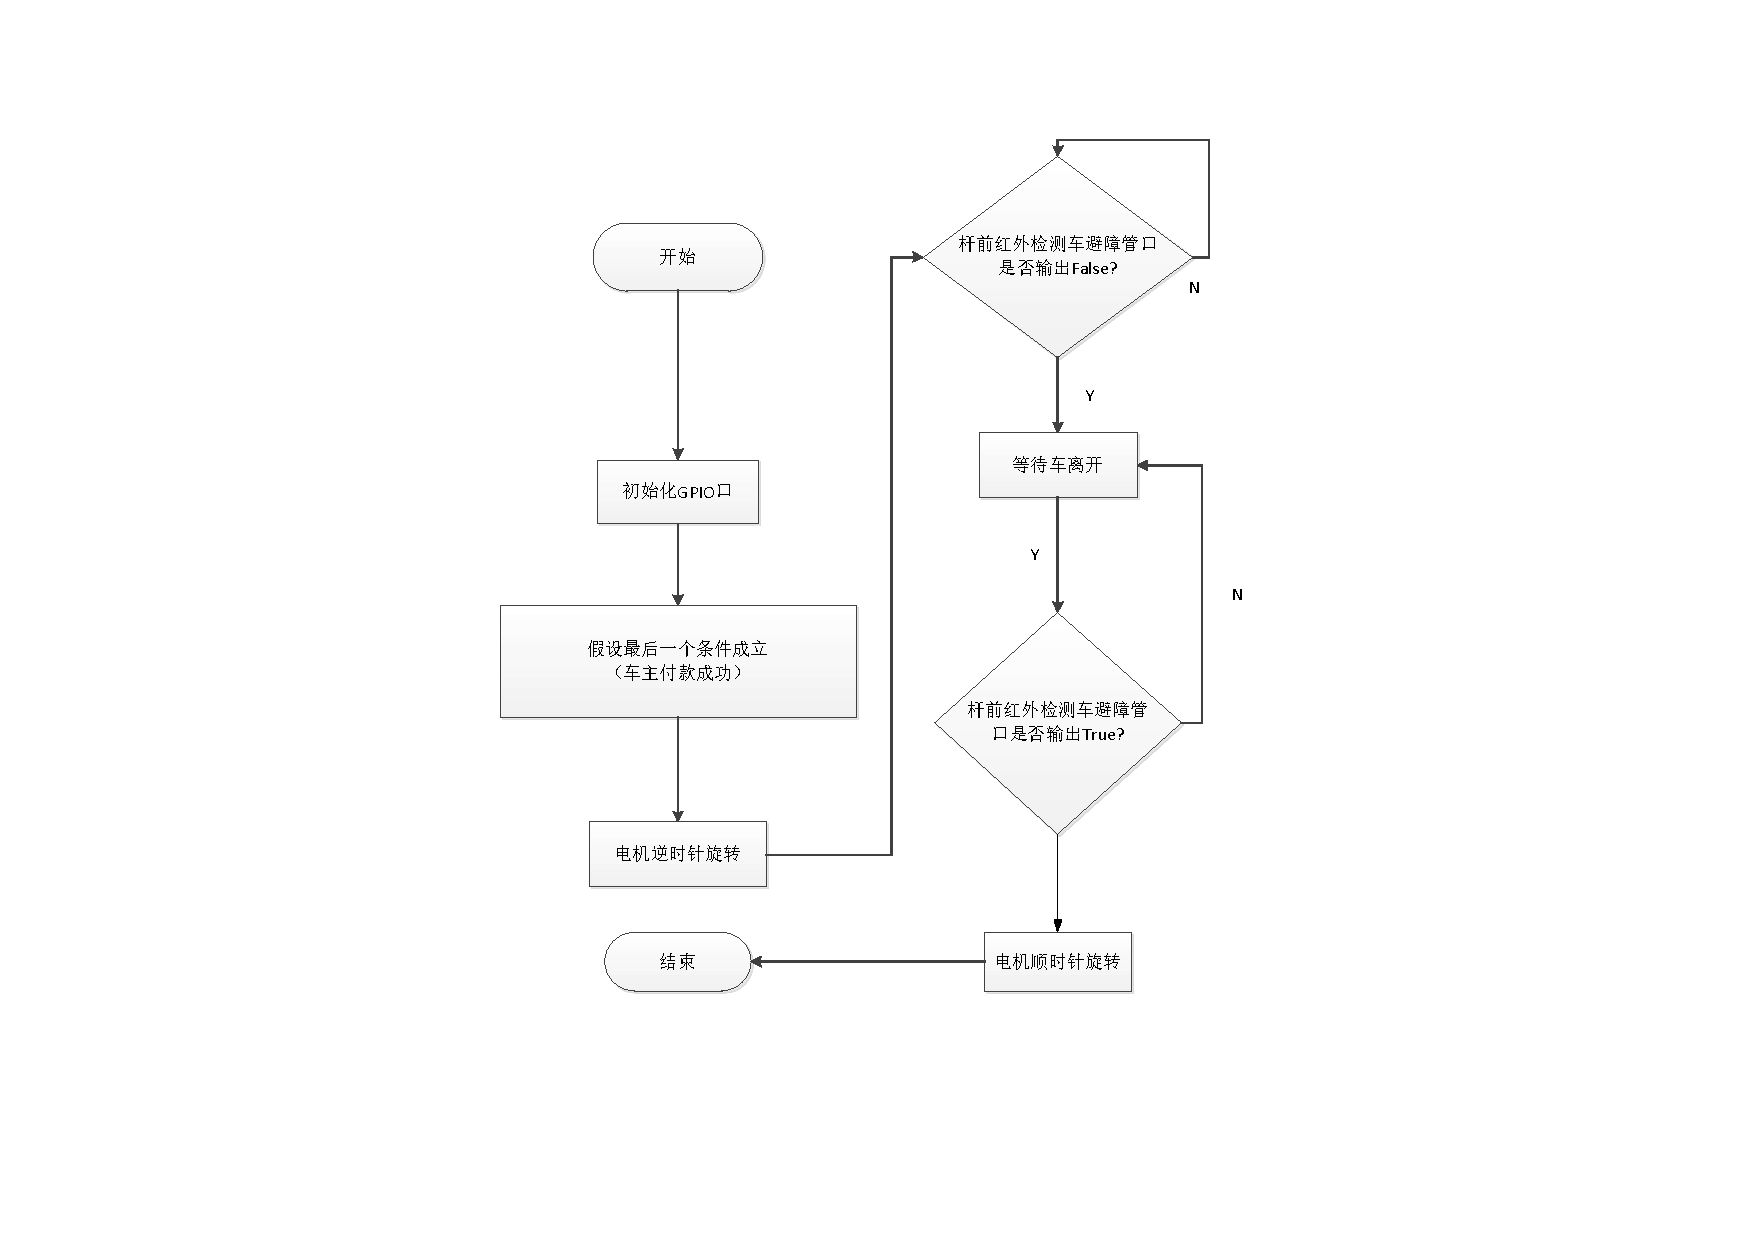
\includegraphics[width=\textwidth]{figure/software-6.pdf}
	\caption{出库驱动模块设计流程图}\label{fig:出库驱动模块设计流程图}
\end{figure}
